\documentclass[12pt]{article}

% Packages
\usepackage{amsmath, amssymb}
\usepackage{graphicx}
\usepackage[margin=1in]{geometry}
\usepackage[backend=biber, style=apa]{biblatex} % Use biblatex with biber
\usepackage{wrapfig}
\usepackage{appendix} % For appendix management
\usepackage{booktabs} % For better table lines
\usepackage{color,soul}
\usepackage{setspace}
\usepackage{hyperref}
%make links look nice
\doublespacing{}
\graphicspath{{../matlab_base/output/}}
% Page layout
\geometry{a4paper, margin=1in}

% Bibliography file
\addbibresource{references.bib} % Specify the .bib file

% Title and Author
\title{\textbf{Impact of an Oil Price Shock on the Canadian Economy} \\ \large{Quantitative Dynamic Macroeconomics}}
\author{Jakub Przewoski, SNR: 2092491\\ Theo Thrän, SNR: 2094766}
\date{\today}
\renewcommand*\abstractname{Executive Summary}
% turning off some linting errors
% chktex-file 3

% ------------------------------------------------------------------------------
% Document
\begin{document}

\maketitle
\pagenumbering{gobble}
% \thispagestyle{empty}

\begin{center}
    \large
    Number of words:
    
    \vfill{}
    \begin{abstract}
        This report analyses the Canadian oil crisis. We calibrate a NK-DSGE model and assume a marginal cost shock. Our findings suggest that the central bank followed a sub-optimal monetary policy rule. Instead, we propose a monetary target rule that incorporates both labour supply and inflation targets. 
    \end{abstract}
\end{center}

\newpage

\tableofcontents{}
% \thispagestyle{empty}

\newpage

\pagenumbering{arabic}
% 2. Introduction
\section{Introduction}
During the late 1970's unrest in Iran leading to the Iranian revolution reduced oil supply significantly\parencite{OilSqueeze1979}. In the early 1980's\footnote{choose which to describe} the countries of the Organization of the Petroleum Exporting Countries failed to agree on quotas, however Saudi-Arabia significantly reduced its production impacting world supply \parencite{tagliabueOPECFAILSSET1982} which was further decreased by the Iran-Iraq war. This caused a worldwide oil crisis. The sharp spike in energy costs across the globe lead to a worlwide recession \parencite{koseGlobalRecessions2020}. During which Canada experienced up to 4\% lower GDP than its long-run trend and inflation increased more than 2\% above its long-run mean 
\parencite{worldbank_inflation_ca,fred_gdp_per_capita_ca}

In this report we evaluate the response of the government to this crisis. We simulate the path of the economy for multiple monetary rules to prescribe the most effective policy that the government could have adopted. We propose a monetary rule that takes into consideration both the deviations of inflation from its steady-state and the deviations of labour supply from the steady-state labour supply. This policy performed the best out of the considered approaches when considered against our benchmark approach in which the central bank can observe the \hl{marginal cost}\footnote{Shouldn't this say shock?} in the economy.

The report is organized as follows: Section~\ref{s:model_description} describes the basic model from which we derive our findings and the parameter calibration. Section~\ref{s:benchmark_model} shows the model simulations with a marginal cost shock (which reflects the oil price shock) and an adjusted monetary policy rule, to reflect the actual events. Section~\ref{s:counterfactual_policy} shows simulations that alternate the strength of the applied policy, and simulations with alternative policy rules. Section~\ref{s:discussion} identifies our prefered policy rule and concludes. 

% ------------------------------------------------------------------------
% THEO ------------------------
% ------------------------------------------------------------------------
\newpage
% 3. Bird’s Eye View of the Model
\section{Bird’s Eye View of the Model}\label{s:model_description}


\subsection*{Model Structure}
% Content here (include figure environment if needed).
The Dynamic Stochastic General Equilibrium (DSGE) Model used for this policy analysis features
three representative agents, namely a representative household, an intermediate goods firm and final goods firm (See grey boxes in figure \ref{fig:model_flow}). The model also includes a government that levies taxes (Figure \ref{fig:model_flow}: yellow box) and can conduct fiscal policy as well as central bank that can conduct monetary policy (Figure \ref{fig:model_flow}: green box).

The representative household aims to maximize its intertemporal utility, which increases with consumption and decreases with hours worked. To do so, it chooses consumption, labour effort, amount of government bonds purchased and investment in capital in every period, taking into account how today's choices affect future outcomes. The household discounts future utility, reflecting a preference for present consumption over future consumption.

The household faces two main constraints. First, it must have cash available to consume, meaning only money saved from the previous period (at 0\% interest) can be used for current consumption. Alternatively, it can purchase one-period government bonds at price $q$, which yield a return of $\frac{1}{q} - 1$ and can be used for consumption two periods later. The household can also invest in capital, earning a capital rent $r$ in the future. Thus, income from labour and capital can be allocated to current consumption, money savings, bond purchases, or capital investment.

Second, the household is subject to a standard budget constraint, requiring that total income is at least as large as total expenses. The allocation between consumption, savings, and investment is made to maximize utility, given these constraints.

In summary, the household's optimization problem involves choosing how much to consume, work, save, and invest each period, balancing immediate utility with future benefits, and operating within the limits of available resources and intertemporal trade-offs.
The representative household aims to maximize its intertemporal utility, i.e.~well-being across all periods.\ It's utility is increasing in consumption and decreasing in hours worked. 

The intermediate goods firm as well as the final goods firm maximize their profit. The revenue of the intermediate firm stem from selling their intermediate good to the final goods firm. The cost incurred consist of the nominal wage paid to labour, rent paid to capital, both of which are provided by the household. It is bound by a Cobb-Douglas production function with a price stickiness friction, and the supply of all intermediate goods must be met by demand for that good from the final good firm.  As just explained the final good firm buys the intermediate goods. It aggregates them into a single final good bought by households and the government. For markets to clear the goods ($Y$) must either be bought by the household for consumption ($C$) or investment ($X$), or the government ($G$). To enforce this the model features a resource contraint (Figure \ref{fig:model_flow}: red ellipsis). The final good firm's input are substitutable to some degree. 

The government has fiscal and monetary policy at their disposal, but cannot combine the two. To represent the shock in energy supply we introduce a exogenous marginal cost shock at the intermediate firm level (Figure \ref{fig:model_flow}: blue box)


\begin{figure}[!h]
    \caption{Model Flow}\label{fig:model_flow}
    \centering
    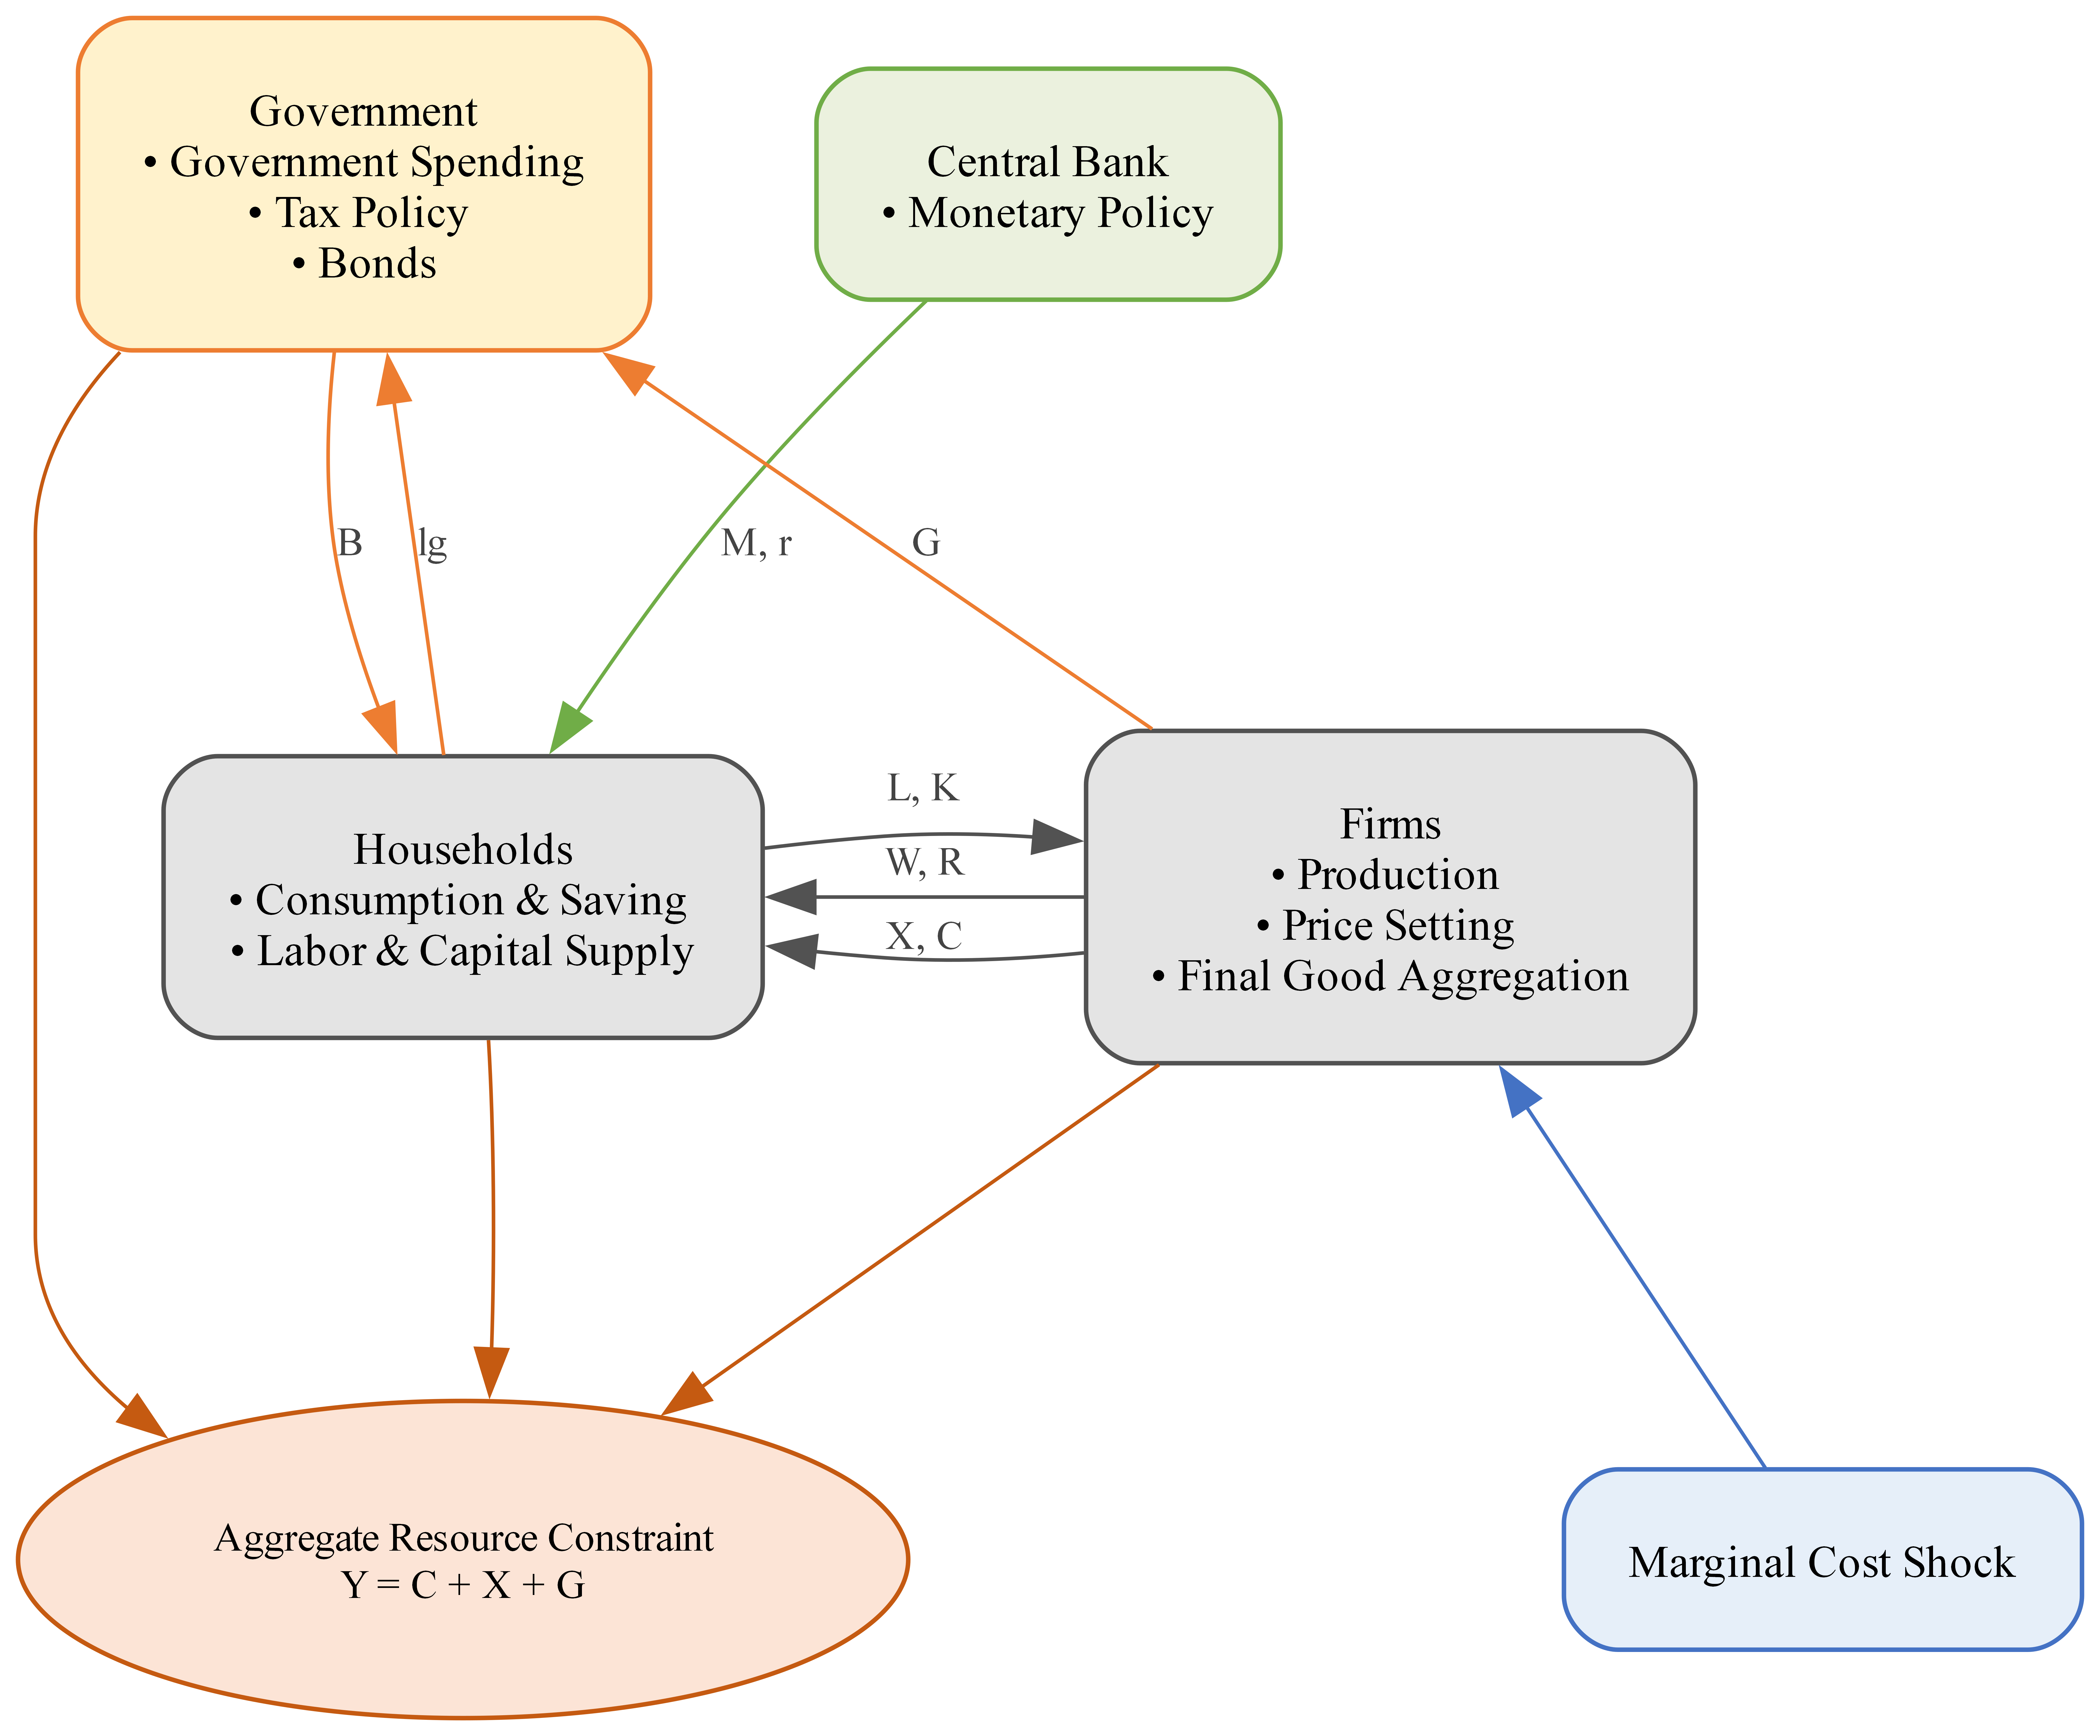
\includegraphics[width=0.8\textwidth]{../../model_graph.png}
\end{figure}

\subsection*{Policy Structure}
The model's default setting assumes that the CB's monetary policy is focused on price stability, i.e. keeping inflation at a target level. The central bank
follows a Taylor-like monetary policy rule, which is a function of the inflation rate and determines the change in the interest rate. We illustrate how monetary policy affects the model economy using the model's default Taylor-like rule which later on is also presented as a counterfactual. If the inflation rate is above the targeted level, the interest rate is decreased and vice versa. The strength of the change in money supply relative to the deviation of inflation is given by the parameter $\theta_{\pi}$. 
The Taylor rule of monetary policy is given by:
\begin{align}
    \frac{1 + r_{B,t}}{1 + \bar{r}_B} = \left( \frac{1 + r_{B,t-1}}{1 + \bar{r}_B} \right)^{\theta_R} \left( \frac{1 + \pi_t}{1 + \pi^*} \right)^{(1 - \theta_R)\theta_{\pi}}
\end{align}

This rule also includes a smoothing term, which means that the change in the interest rate is not only a function of the current inflation rate but also of the previous period's interest rate. The parameter $\theta_R$ determines how much the central bank smooths its interest rate changes, i.e. the inertia of monetary policy. A value of 0 means that the central bank does not smooth its interest rate changes at all, which is the assumption in the counterfactual scenario. 

So when the central bank observes a deviation of inflation from its target, it adjusts the interest rate accordingly. This change in the interest rate in turn influences consumption and investment decisions of the household and firms. When the interest rate is higher it becomes more attractiv to buy bonds as their payoff next period is higher. Thus, consumption tomorrow is reduced as the household saves less in money holdings and more in bonds. The same logic applies to investment, when the bond return is higher, relatively the return on capital is lower, thus the household invests less in capital.
% The central bank's goal is to stabilize inflation around its target level, which is set at 0\% in this model.

The fiscal policy rule works similarly\footnote{Should we include a fiscal policy rule as alternative policy?}, but instead of the central bank changing the interest rate the government adjusts a variable tax surcharge ($\tau_t$). This surcharge is added to the individual tax rates for labour income, capital income and consumption. This surcharge is a function of the level of government debt ($l_{g,t}$) and the steady-state target level of government debt ($l^{\star}_{g}$). The government reacts to the difference between the two levels of government debt by adjusting the surcharge. If the debt level is above its steady state target the surcharge is increased above its steady state level and vice versa. The incremental change of the surcharge is guided by a parameter $\lambda_{l g}$, which determines how responsive the government is to the deviation of government debt from its target. The fiscal policy rule is given by:
\begin{align}
    \tau_t - \tau^{\star} = \lambda_{l g} (l_{g,t} - l^{\star}_{g})
\end{align}

The outstanding government debt is given by the outstanding bonds and currency in real terms. The government debt changes by the difference between government spending ($G_t$) and tax revenue (taxes + surcharge on $C_t, K_t, w_t,L_t$) adjusted for the bond interest rate. The government spends on the aggregate good provided by the final goods firm. Furthermore, if inflation is positive the real value of bonds issued last periods is decreased and thus reduces government debt.

% Content here (use align or equation environments).

\subsection*{Calibration}
The model is calibrated to the Canadian economy in 1979\footnote{See table \ref{tab:parameters} in the appendix for a concise overview}, assuming that one period corresponds to a year. 
The discount factor $\beta$ is set to 0.96, inline with \textcite{someOilDemandSupply2023} and close to \textcite{corriganToTEMIIIBank2021}. 
The intertemporal consumption elasticity $\sigma$ is set to 2. Positive values indicate risk-aversion, whereas a negative value would correspond to risk-loving behaviour
\parencite{thimmeIntertemporalSubstitutionConsumption2017}.

Estimates for the inverse Frisch elasticity $\gamma$ differ starkly, between macro and micro estimates. Reasons for this discrepancy
include that micro studies use a sample which constitutes a subset of the population (e.g.\ primary earners, in the midst of their careers) whereas macro 
estimates try to copy behaviour of the entire population. Furthermore, micro estimates usually do not consider the extensive margin, i.e.\ the decision 
to work or not. Since the model attempts to capture macro trends we use a macro estimate of 3 \parencite{petermanReconcilingMicroMacro2016}. 

Money velocity $\nu$ is calculated, using Fisher's quantity equation, as the ratio of nominal GDP to the money stock (M1) (with data from: \textcite{bankofenglandCanadianDollarData2021}; 
\textcite{federalreservebankofminneapolisInflationCalculatorFederal}; \textcite{worldbankgroupWorldBankNational}; \textcite{bankofcanadaSelectedMonetaryAggregates})\footnote{GDP from World Bank in 2015 USD converted to 1979 USD using Federal Reserve Minneapolis, converted to CAD using historic annual average exchange rate from 
the Bank of England, Money Supply from Bank of Canada.} yielding 4.2. Thus, $\nu$ is set to 1/4.2 = 0.24. 

The capital depreciation rate $\delta$ is set to 0.1, matching the estimate of \textcite{statisticscanadaDepreciationRatesProductivity2007} and the calibration in \textcite{someOilDemandSupply2023} and \textcite{corriganToTEMIIIBank2021}.
The capital share of income $\alpha$ is set to 0.31~\parencite{fredst.louisShareLabourCompensation2021,feenstraNextGenerationPenn2015}. 
\footnote{The elasticity of substitution between differentiated goods, even though a parameter of the final goods firm is not really a production process parameter. 
Rather, it aggregates all goods into a single consumption good and thus is better understood as an elasticity of substitution between consuming differentiated goods.}. 

The three tax-rates are set in accordance with the average effective tax rates in Canada in 1980--1985. The labour income tax rate $\tau_L$ is set to 0.24, the capital income tax rate $\tau_K$ is set to 0.25 and the consumption tax rate $\tau_C$ is set to 0.13
\parencite{careyAverageEffectiveTax2000}. 

Price stickiness parameter $\kappa$ and the investment adjustment cost parameter $\phi_X$ are set to 120 and 12 respectively to increase the model's fit to the data\footnote{ We do not use a formal minimization process but rather visually inspect the best-fit.}. As data, we use the deviation of inflation from its long-run (1961--2024) average ($\bar{\pi} =  3.72$)~\parencite{worldbank_inflation_ca}. To identify the deviation of GDP from its steady-state we use the one-sided Hodrick-Prescott filter, identifying the cyclical component of GDP \parencite{fred_gdp_per_capita_ca}. The chosen values of $\kappa$ is twice as large as the default, meaning that prices are sticker because (the intermediate) firms are more reluctant to change prices. This is enforced due to a penalty deducted from the intermediate firm's output regualted by $\kappa$. $\phi_x$ works similar but rather regulates the penalty given to households for changing their investment choice, by reducing the pass-through from investment to the capital stock. So the increase in both parameters reflects higher levels of inertia for price-setting and investment decisons. 

The persistency parameter of the shock ($\rho_{sMC}$) described in section~\ref{s:benchmark_model} is set to 0.5, while its standard deviation ($\sigma_{sMC}$) is set to 1. A more thorough analysis of these choices would be valuable in the future.
% ------------------------------------------------------------------------
% ------------------------------------------------------------------------

% 4. Benchmark Model Analysis
\newpage
\section{Benchmark Model Analysis}\label{s:benchmark_model}

In this section, we adjust our model to replicate the policy carried out by the Bank of Canada (BoC). To reflect the change in the behaviour of the central bank, we modify the Taylor-like rule to a money supply target. Following the behaviour of Bo, the money supply rule is based on the deviations from the steady-state inflation rate. Therefore, it implies a focus of the bank on achieving price stability. Equation~\ref{eq:baseline_rule} displays the rule min formal notation.


\begin{equation}\label{eq:baseline_rule}
    \frac{M_t}{M_{t-1}} = \Big(\frac{1+\pi_{t}}{1+ \bar \pi}\Big)^{-\theta_{\pi}}
\end{equation}

We specify the $MC$ shock to enter the model through the Phillips curve. That is because the curve represents the pricing decision rule of the intermediate companies, and so it will most accurately represent their reaction to an increase in marginal costs. Equation~\ref{eq:phillips_curve} shows the NK-Phillips curve adjusted for our shock. 

\begin{equation}\label{eq:phillips_curve}
    \frac{\kappa \pi_t (1 + \pi_t)}{1 - \frac{\kappa}{2} \pi_t^2}
    = \frac{1 - \frac{\rho}{mc_t \cdot e^{MC_s,t}}}{1 - \rho}
    + \mathbb{E}_t \beta_{t,t+1}
    \frac{Y_{t+1}}{Y_t}
    \frac{mc_{t+1} \cdot e^{MC_{s,t+1}}}{mc_t \cdot e^{MC_s,t}}
    \frac{\kappa \pi_{t+1} (1 + \pi_{t+1})^{2}}{1 - \frac{\kappa}{2} \pi_{t+1}^2}
\end{equation}

Where the periodic shock is expressed multiplicatively as $mc_t \cdot e^{MC_{s, t}}$ for convenient estimation.

\subsection*{Economic Fluctuations Induced by the Shock}

This specification leads to the fact that in the period of the shock, intermediate firms will adjust their prices and revise their hiring decisions. The economic intuition behind this is that an increase in marginal costs, decreases the markup of the firm which then chooses to adjust its prices. As adjustment is costly (due to $\kappa$), the firms will raise their prices less than the increase in marginal costs. In turn, higher prices, cause a decrease in demand for the aggregate product, therefore prompting the firms to decrease output. At the same time, the higher marginal costs imply that the companies choose to hire less labour and capital, as it becomes more costly. Furthermore, the high prices and lower output imply a fall in real wages and the real rental rate of capital.

The $mc_t \cdot e^{MC_{s, t}}$ feeds into firms' expectations about the future. When firms choose to set their prices for $t$, they trade off increasing their prices today and in the future. If the shock is expected to be persistent, firms may choose to increase their prices by less in $t$ and choose to keep increasing them slowly over time. 

The firm's pricing decision is also important for their future behaviour, as it is used as a benchmark relative to which they set their next prices in the next period. 
% If prices are set high in period $t$,\ \dots\footnote{Does it increase the costs of raising the prices later on??? I don't think so}

Over time, as no more shocks happen, firms are able to arrive back at their target markup and therefore the economy is able to come back to the steady state inflation rate. This also implies that the intermediate firms slowly come back to their steady state hiring decisions, and households again arrive at their steady state consumption.\footnote{Adjust/Expand on this part.}

% describe the short run as well as the path back to the steady state. 
\subsection*{Idea of the Implemented Policy}

At the same time, in an effort to counter inflation, the central bank will decrease the money supply which acts analogously to a rise in the interest rate. A reduction in the money supply of households, implies a decrease in purchasing power, which translates into lower output in the given period. However, the decrease in demand incentivizes the firms to slow down the growth in their prices (or even decrease them if the drop in demand is large enough). The reduction in demand further causes firms to revise their hiring decision in favour of lower production. Over time this policy leads to a rapid reduction in inflation and a slow recovery in output.

\subsection*{Impulse Response Functions and Model Limitations}

Figures~\ref{fig:main_baseline} and~\ref{fig:other_baseline} display the impulse response functions of the baseline model. Figure~\ref{fig:main_baseline} displays the IRF's for real GDP, inflation and the total hours worked ($L$). The blue curve shows the path of the economy as simulated by our model, while the red curve displays the path of the economy according to the empirical data.\footnote{We restricted ourselves to showing only the comparison for GDP and Inflation, as we couldn't find the labour data.} As one can see, our model approximates the true crisis, however there remain some limitations. Following the shock to marginal costs we can see a drop in output and a rise in prices in the short term. The focus of the central bank on managing inflation causes it to over-contract, which results in the deflation visible in the medium-run. Moreover, one can see total hours worked drop rapidly as described in the above section. 

Figure~\ref{fig:other_baseline} displays the IRF's for the rest of the variables. Similarly to the total hours worked, we can see that capital employment falls following the shock. The shock has larger implications for the whole of the economy with virtually all of the observable variables falling following the shock: wages, return on capital, consumption, investment. 

\begin{figure}[!h]
    \caption{Impulse response functions of observable variables}\label{fig:main_baseline}
    \centering
    \includegraphics[width=0.7\textwidth]{main_baseline_policy.png}
    
    \tiny{Data source: \citeauthor{worldbank_inflation_ca}}
\end{figure}

Finally, the last row of Figure~\ref{fig:other_baseline} displays the effects on the interest rate, real marginal costs and money stock. Whereas the effects on the real marginal costs are straightforward and as specified by our shock process, the effects on the nominal interest rate and the money stock are of interest. The panel on money stock shows the drastic short-run contraction carried out by the central bank. The panel displaying the path of the interest rate shows a large drop relative to the steady state value in the shock period and an increase in the periods following. This can be explained by considering the effects of the shock on households. In the initial period, household face high prices, and low consumption. As they are aware of the inner workings of the economy (namely the monetary policy rule as well as the persistence of the economic shocks), they can expect both high inflation, low consumption and further contractions in the short term and a slow recovery in the medium term. Therefore, they initially choose to postpone more of their consumption using the purchases of bonds, which pushes the interest rate down relative to its steady state. 

\begin{figure}[!h]
    \caption{Impulse response functions of observable variables}\label{fig:other_baseline}
    \centering
    \includegraphics[width=0.7\textwidth]{other_baseline_policy.png}
\end{figure}

Overall, although this model approximates the crisis, it misses certain aspects of history. Firstly, it misses the international effects of the crisis. Although the recession was worldwide, the impact of other nations on the demand for exports from Canada could have had an effect on the economy during the crisis, whereas here it is entirely excluded, given that we operate within the closed-economy framework. Furthermore, at this point in time, the Canadian Dollar has been floating freely against other currencies, which naturally could have had effects on the economy through the general stabilization that the floating exchange rates offer. Moreover, although our model follows the general direction of the economy, it fails to precisely approximate the realized path. This is likely due to the noise included in the empirical data, differences in policy specification and the use of impulse response functions. The noise can be inferred from the large volatility of our data. As can be seen in Figure~\ref{fig:main_baseline}, the original policy may have been specified differently as the economy avoided deflation. Finally, while our impulse response functions assume no repeated/other shocks, the empirical data does not conform to this assumption, with other shocks (such as those related to international finance) possibly impacting the economy.

\newpage
% 5. Counterfactual Policies
\section{Counterfactual Policies}\label{s:counterfactual_policy}
In this section we consider various alternatives to the policy chosen in initial scenario.

\subsection*{Counterfactuals with Different coefficents}

Figure~\ref{fig:policy_par_variation} considers variation in responsiveness of the central bank to inflation (using the initial policy). As can be seen on the graph, choosing different values for $\theta_{\pi}$ has a significant impact on the economy, with the contraction in real GDP and the total hours worked both being increasing in the parameter. At the same time, an increase in the parameter does not seem to be causing a significant change to the inflation experienced by the economy. This happens, because the stronger change in the money supply (if $\theta_\pi$ increases) impacts the consumption and labour choice of households, however it does not change the price setting behaviour of firms due to the price-stickiness. Therefore, policy that is more strongly focused on preventing inflation, will result in the economy contracting more, while maintaining similar inflation levels.

\begin{figure}[!h]
    \caption{Impulse response functions of observable variables}\label{fig:policy_par_variation}
    \centering
    \includegraphics[width=0.7\textwidth]{policy_par_variation.png}
\end{figure}


\subsection*{Counterfactuals with Alternative Policies}

In this subsection we consider other monetary policy rules that the central bank could have followed instead. We consider the following rules:

\begin{equation}\label{eq:mc_rule}
    \frac{M_t}{M_{t-1}}
          = \Big(\frac{mc_t}{\bar{mc}}\Big)^{-\theta_{mc}}
            \cdot \Big(\frac{1 + \pi_t}{1 + \bar{\pi}}\Big)^{-\theta_{\pi}}
\end{equation}

Equation~\ref{eq:mc_rule} is our benchmark policy that relates the money supply target to both the relative value of marginal cost and inflation. In this regime, the central bank observes the shock to the marginal cost directly, and tries to balance the impact to the economy of the $mc$ and inflation. We consider this our ``first-best'' scenario, as observing the marginal cost in real time is difficult and might not be realistic, while also being specific only to economies plagued \textit{only} by marginal cost shocks.

\begin{equation}\label{eq:lab_rule}
    \frac{M_t}{M_{t-1}}
        = \Big(\frac{L_{t-1}}{\bar{L}}\Big)^{-\theta_L}
          \cdot \Big(\frac{1 + \pi_t}{1 + \bar{\pi}}\Big)^{-\theta_{\pi}}
\end{equation}

Equation~\ref{eq:lab_rule} displays the same idea, but with respect to labour. In this scenario, the central bank tries to manage both the impact on inflation and the labour market, therefore following a U.S. Federal Reserve-like mandate, where the bank also tries to maintain full employment. However, in this scenario, the central bank considers the labour supply of previous period when increasing the money supply. This is for two reasons: firstly, consumption today is determined by the labour yesterday. Therefore, it makes more sense for the central bank to adjust the money target, and thus the lump sum payment to the households, based on the previous value. Secondly, if the central bank were to set the monetary target based on the labour today, it would only be impacting the consumption tomorrow, which takes away the power of monetary policy.  

\begin{equation}\label{eq:taylor_rule}
    \frac{1 + r_{B,t}}{1 + \bar{r}_B} = \left( \frac{1 + r_{B,t-1}}{1 + \bar{r}_B} \right)^{\theta_R} \left( \frac{1 + \pi_t}{1 + \pi^*} \right)^{(1 - \theta_R)\theta_{pi}}
\end{equation}

Finally, we also consider equation~\ref{eq:taylor_rule}, which is the previously shown interest rule. We display it as an example of the performance of the basic model.  


Figure~\ref{fig:policy_rule_variation} displays the effects of different monetary policies. As described above, equation~\ref{eq:mc_rule} acts as our benchmark, as it performs the best and allows for the economy to come back to the steady state the earliest. This is due to the fact that if the central bank is able to observe the shock directly, it can respond in each period to the precise value of the marginal costs.

Equation~\ref{eq:lab_rule} performs as the second-best. In the initial period this rule performs poorly, as the central bank is backward looking in this regime, and therefore only takes into consideration the inflation that it observes in that period.  

\begin{figure}[!h]
    \caption{Impulse response functions of observable variables}\label{fig:policy_rule_variation}
    \centering
    \includegraphics[width=0.7\textwidth]{policy_rule_variation.png}
\end{figure}

However, over time, it is able to bring the economy back to the steady state in the second-fastest manner, by taking into consideration the effects of the shock on labour supply. This happens, because as the central bank sees that the labour supply in previous period was low, it is able to infer that the savings of the households will be smaller, and therefore they will not be able to consume as much as they would have in the absence of the shock. Thus, the central bank increases their purchasing power in that given period. It is important to note that this happens at the expense of a slightly higher inflation before returning to the steady-state. Furthermore, this policy works well if the shocks are infrequent and persistent, however if the economy is troubled by many short-lived shocks, it may be unsuitable as then the central bank would repeatedly fail to anticipate it.

Equation~\ref{eq:taylor_rule} presents itself as marginally better than the implemented equation~\ref{eq:baseline_rule}. As the parameter $\theta_R$ is assumed to be $0$, the interest rate rule, essentially acts in the same way as equation~\ref{eq:baseline_rule}, with interest-rate targeting based on the inflation deviations. However, as the instrument of choice is the interest rate setting, the effect on the economy is more measured, because it doesn't directly impact consumption. This rule instead acts on the trade-off between future money and bond savings, which results in a more moderate reduction in output and higher inflation. Nonetheless, both of these policy rules present a scenario in which the economy sharply contracts (yet less than under the labour rule), and takes longer to come back to the steady-state. 

Finally, the implemented equation~\ref{eq:baseline_rule}, causes a hard contraction in output, high inflation (followed by deflation) and a sharp decrease in labour supply. This is caused by the fact that the central bank focuses solely on the inflation target. Unlike the other policies, this instrument causes a temporary deflation, which happens because of the drastic action taken by the central bank and a lack of consideration for other variables.




% -------------------------------------------------------
% 6. Policy Recommendation and Discussion
\section{Policy Recommendation and Discussion }\label{s:discussion}

As shown by Figure~\ref{fig:policy_rule_variation}, there is a trade-off between the speed at which GDP recovers and the initial level of inflation. Based on our simulations, we identify money supply targeting based on the deviation of labour and inflation from their steady-state levels as the second-best policy, and thus as the policy that should have been pursued. We deem it the second-best because it has GDP and employment reach the pre-shock level fastest, whilst having lower initial inflation than the benchmark and reaching the pre-shock inflation level at a similar speed to the other tested policies. Nonetheless, the second-best policy performs significantly better than interest rate or money supply targeting based solely on inflation. The first-best policy, which targets marginal costs directly, is deemed unfeasible as outlined above. 

However, the fast recovery of GDP comes at two cost. First, the initial decrease in GDP is significantly larger and initial inflation is higher and recovers slower than when policies that solely react to inflation are implemented. The former leads us to caveat our recommendation that this policy is not suitable for an economy, exposed to frequent shocks as the speedy recovery is outweighed by the initially larger drop of GDP. 

Based on our analysis we conclude that, in the presence of large supply shocks, central banks should consider monetary policy rules that respond to both inflation and real activity (such as labour), rather than focusing exclusively on inflation. This approach allows for a faster recovery in output and employment, albeit at the cost of temporarily higher inflation. The results suggest that a dual-mandate approach, similar to that of the Federal Reserve, would have been more effective in stabilizing the Canadian economy during the crisis period under study. This recommendation is under the limitations of the model outlined above and furthermore limited by the number of policies tested, as well as that we test counterfactual policies only for a single policy parameter. 

The superiority of the dual-mandate policy in our simulations is not surprising, given the absence of an active fiscal policy to complement a single-mandate monetary policy. In real-world scenarios, when monetary policy is focused solely on inflation, fiscal policy can stabilize output and employment during supply shocks. For example, during the 2022 European energy crisis (a similar shock to the one studied), many European countries responded to the supply shock with a combination of expansionary fiscal policy and increased interest rates \parencite{bankoffinlandEuropeanCentralBanks2022, checherita-westphalUpdateEuroArea2023}. This coordinated approach helped to cushion the impact on GDP whilst addressing inflationary pressures.
%references
\newpage %start a new page
\printbibliography{} % Print the bibliography

% Appendix 
\newpage
\appendix
\section{Appendix}
\begin{table}[ht]
    \centering
    \caption{Parameter Calibration}\label{tab:parameters}
    \begin{tabular}{cll}
        \toprule
        Parameter & Description & Value  \\ \midrule
        %\hline \hline
        $\beta$ & Period discount factor  & 0.96  \\
        $\sigma$ & Intertemporal consumption elasticity  & 2  \\
        $\gamma$ & Inverse Frisch elasticity  & 3  \\
        $\nu$ & Money velocity  & 0.24  \\
        $\delta$ & Capital depreciation rate  & 0.1  \\
        $\phi_X$ & Investment adjustment cost parameter & 12  \\
        $\alpha$ & Capital share of income & 0.31  \\
        $\rho$ & Elasticity of substitution for differentiated goods &  0.8  \\
        $\kappa$ & Price stickiness & 60 \\
        ${\tau_L}$ & Labour income tax & 0.24 \\
        ${\tau_K}$ & Capital income tax & 0.25 \\
        ${\tau_C}$ & Consumption tax & 0.13 \\
        $\sigma_{sMC}$ & Standard deviation of shock & 1 \\
        $\rho_{sMC}$ & Persistency of shock & 0.5 \\
    \bottomrule
    \end{tabular}
\end{table}

\end{document}